\chapter{\expUser}
\label{sec:userstudy}

\ref{sec:design_workshop}장에서 우리는 `\concept'\를 전달하는 시스템 \sysname의 핵심 요소와 모듈들을 제시했다. 본 장에서는 \sysname\을 오즈의 마법사(Wizard-of-Oz) 형태로 사용자들에게 체험하도록 하여 그 효과를 관찰하고자 한다.

본 장은 다음과 같이 구성된다. 첫째, 시나리오 기반의 실험 설계 과정에 대해 이야기한다. \concept\를 체험할 수 있는 실험 환경 구성의 어려움과, 이를 실험 디자인 과정에서 다룬 방법을 서술한다. 둘째, 실험에 참여한 피험자 부부들의 특성에 대해 서술한다. 총 5팀, 10명의 사람들이 참여했으며, 이들 부부가 어떻게 평소에 시간을 같이 보내는지 얘기한다. 마지막으로 실험을 통해 관찰한 결과를 다룬다. \sysname\ 디자인 과정에서 고려한 요소들이 실제 사용자 실험에서 어떻게 나타났는지 얘기한다. 본 실험은 IRB 승인(KH2017-18) 아래 진행했다.


%%%%%%%%%%%%%%%%%%%%%%%%%%%%%%%%%%%%%%%%%%%%%%%%%%%%%%%%%%%%%%%%%%%%%%%%%
\begin{figure}
\begin{subfigure}{.5\textwidth}
  \centering
  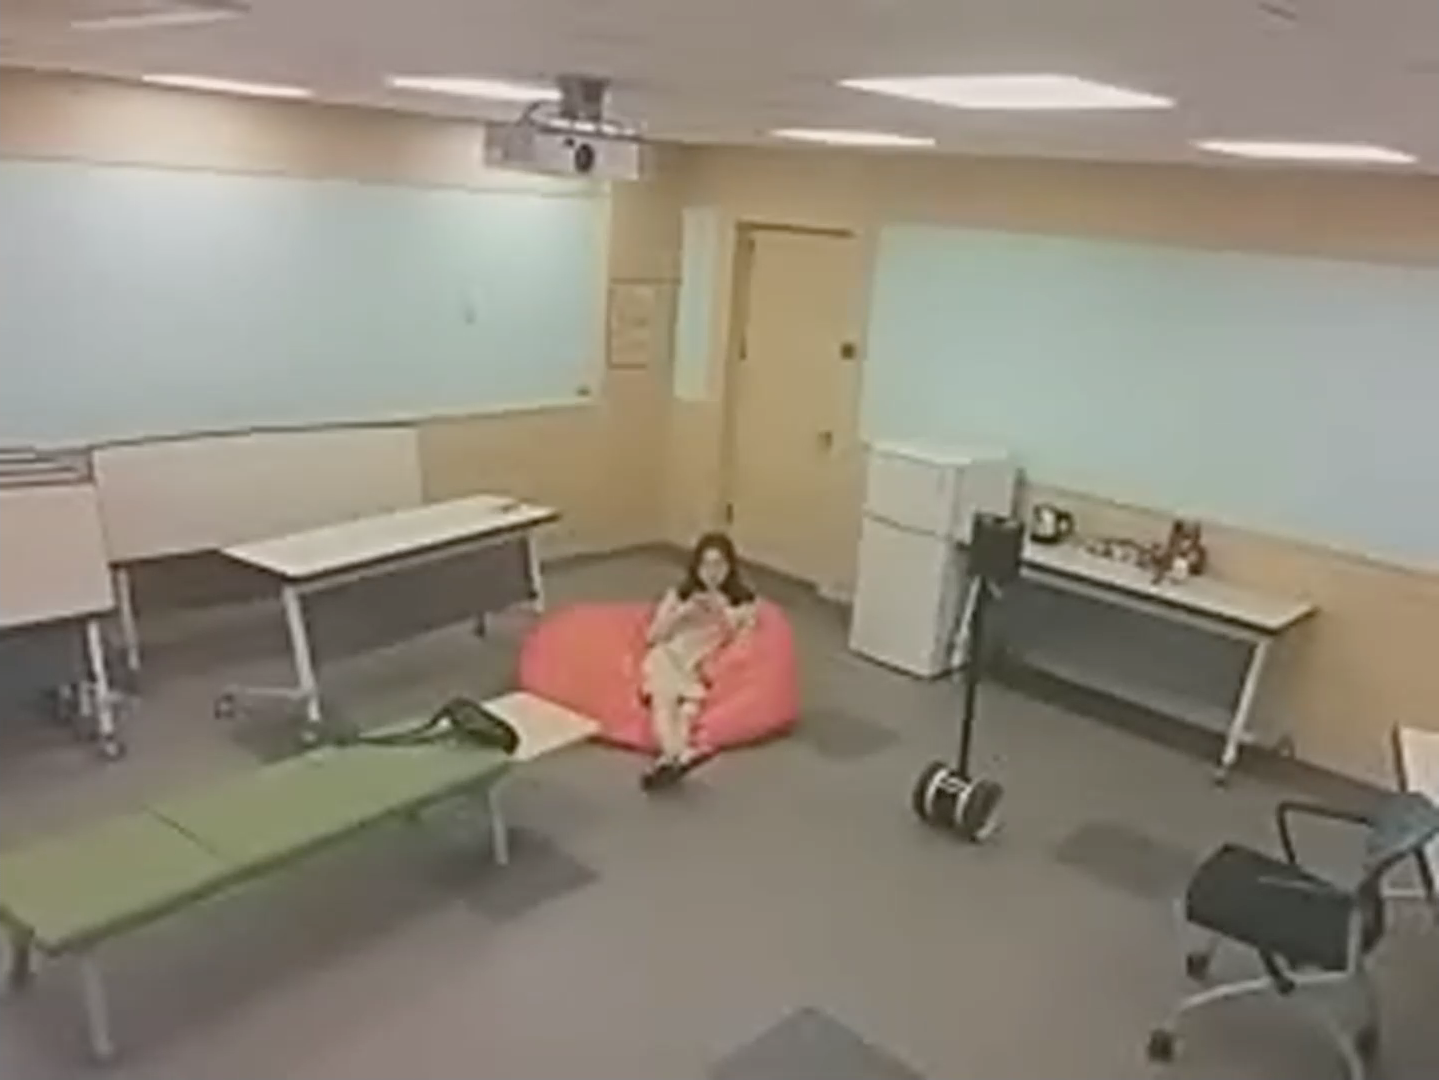
\includegraphics[width=0.9\textwidth]{images/sceneA}
\end{subfigure}
\begin{subfigure}{.5\textwidth}
  \centering
  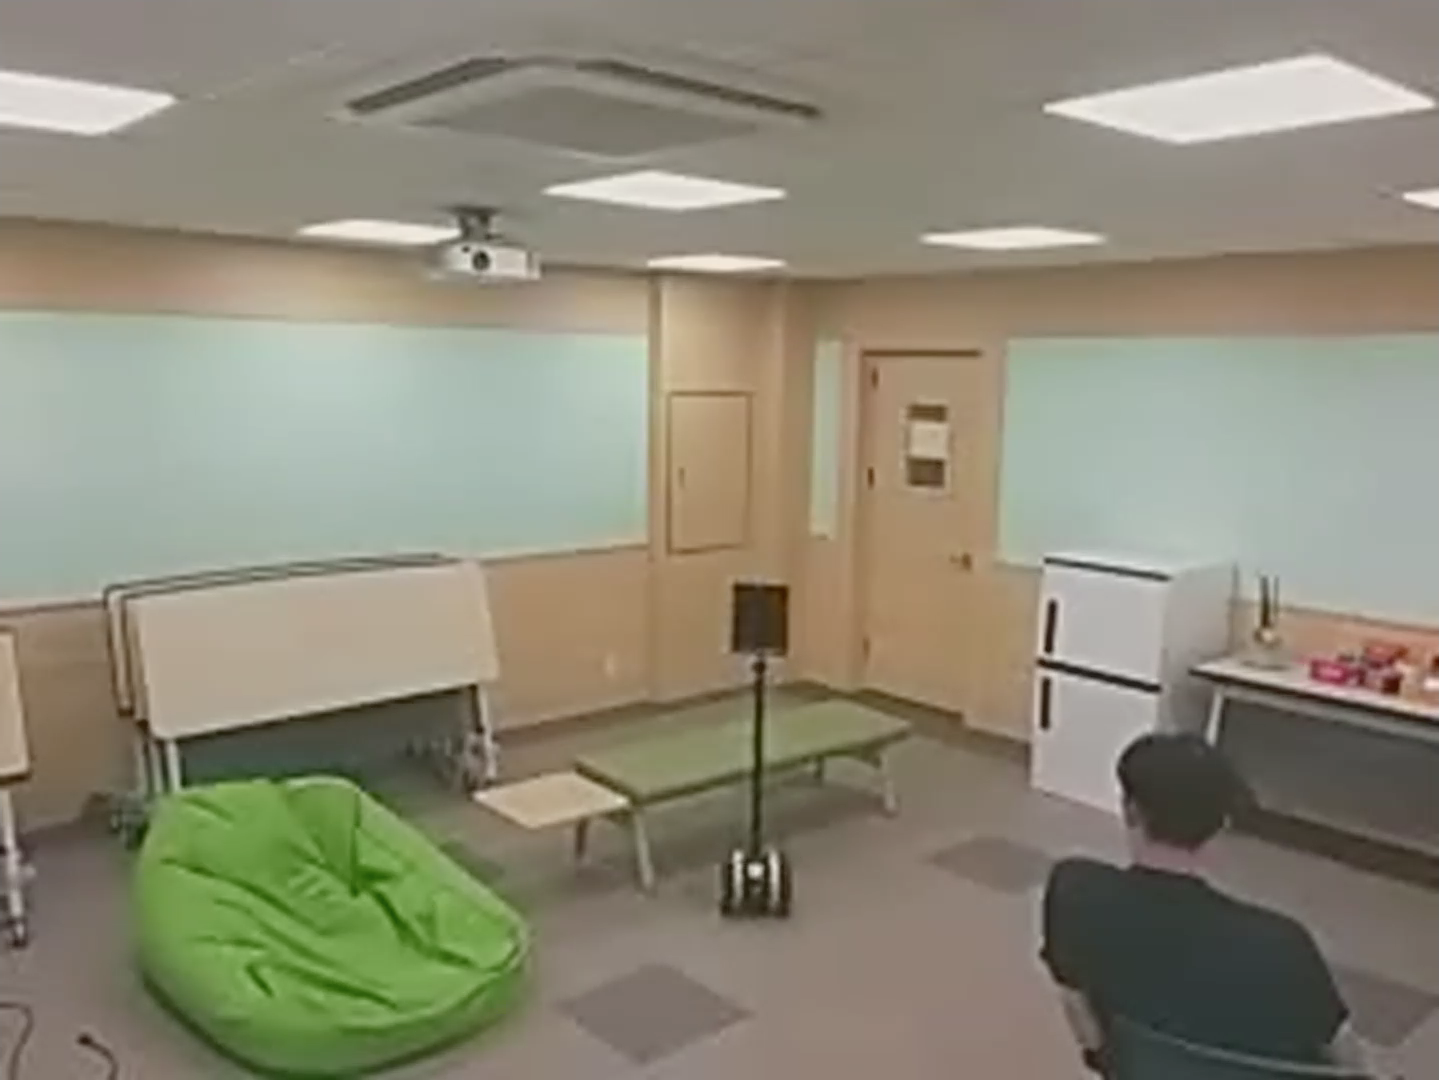
\includegraphics[width=0.9\textwidth]{images/sceneB}
\end{subfigure}
\caption{랩 환경에서 진행된 시나리오 중심 사용자 스터디 실험 장면}
         % 로봇 아바타는 상대방의 의미적 위치로 지속적으로 이동하며 두 방 사이를 연결짓는다.
\label{fig:userstudy_scene}
\end{figure}
%%%%%%%%%%%%%%%%%%%%%%%%%%%%%%%%%%%%%%%%%%%%%%%%%%%%%%%%%%%%%%%%%%%%%%%%%


\section{실험 디자인}

% 은근한 함께 삶의 섬세함
`\concept'\는 섬세한 감각이다. 일상 속, 익숙한 공간에서 시간을 함께 보낼 때 생겨나는 미묘한 감각을 실험 환경 속에서 포착하기 위해서는 실험 또한 섬세하게 디자인되어야 한다. 본 장에서는 \concept\를 실험하기 위한 디자인으로 \expUser\를 제시한다. 또한 섬세한 감각을 실험실 환경에서 재현하기 위해 어떠한 과정을 거쳤는지 서술한다.

\subsection{목표}
\label{subsec:exp_goal}

우리는 앞서 \ref{sec:concept}장에서 \concept\를 형성할 때 필요한 5가지 핵심 상태에 대해 얘기했다.

\begin{center}
\begin{minipage}{.6\textwidth}
\begin{enumerate}[label=\Roman*., noitemsep]
	\item 상대방이 나와 같은 공간에 있다고 인지할 수 있는 상태
	\item 상대방의 상황(상태)을 언제든지 파악할 수 있는 상태
	\item 상대방이 나를 의식한다는 것을 인지하고 있는 상태
	\item 언제든지 상대방과 소통할 수 있는 상태
	\item 서로의 활동을 방해하지 않고 있는 상태
\end{enumerate}
\end{minipage}
\end{center}

\noindent 본 실험의 목표는 우리가 제시하는 \sysname\이 위에 나열된 상태의 형성에 어떤 도움을 주는 지 확인하는 것이다. 실제 함께 살아가는 사람들 사이에서 \concept\가 어떠한 형태로 나타나는 지 확인하고, 해당 순간에 컴퓨터 기술이 어떻게 녹아들 수 있는 지 보이고자 했다.


\subsection{실험 방법}

% 실험 방법 Overview
실험은 사전 인터뷰, 시나리오 체험, 사후 인터뷰 순서로 수행하였다.
먼저 \concept\와 관련된 피험자들의 의견을 수집하기 위해 약하게 구조화된 인터뷰(Semi-structured Interview)를 수행했다. 인터뷰를 통해 커플의 인구학적 특성 및 실제 일상생활에서 \concept\를 느끼는 순간들에 관해 조사하였다.
실험참가자들은 이후 집안 환경을 모사하여 꾸민 방으로 이동했다. 참가자들은 시험 공부, 드라마 시청, 여행 계획 세우기 등 미리 준비해온 업무를 수행하며 일상적인 시간을 보냈다. 동시에 참가자들은 영상 통화 및 \sysname\을 통한 연결을 체험했다.
사후 인터뷰 세션은 시나리오 체험 시간 동안 관찰된 행동을 중심으로 진행했다. 각 연결 기술의 사용자 경험의 차이와 특이 행동에 대한 참여자의 주관적 해석을 중점적으로 조사하였다.
전체 실험은 이틀에 걸쳐서 이루어졌다. 각 실험은 1시간 40분에서 2시간 길이로 진행했다.

인터뷰 자료 분석은 실험 종료 후 진행했다. 실험 결과는 녹취록 및 영상 자료로 정리 된 후 공동 연구자들에 의해 여러 번 검토되었다. 이후, \ref{sec:concept} 장에서 언급한 테마를 기반으로 관찰 결과를 정리했다.


\subsubsection{실험 참가자 모집}

실험 참가자들은 대학교(KAIST)내 구성원 커뮤니티 웹사이트에 모집 광고를 게시하여 모집하였다. 총 7쌍의 커플이 지원했으며, 이들 중 나이와 부부 형태의 다양성을 고려하여 5쌍을 선택했다. 참가자의 직업의 경우 대학원생의 비율이 높았지만, 해당 직업군은 떨어져 사는 생활을 경험하는 비율이 높기에 초기 연구에 적합하다고 보았다. 실험 참가자들은 함께 살아온 시간이 3개월 이상인 그룹으로 제한하였다. \concept\를 느끼기 위해서는 서로의 생활에 대한 깊은 이해가 필수적이므로, 일정기간 이상의 시간을 함께 보내는 것이 필요하다고 고려하였다. 총 10명의 실험 참가자에 관한 정보는 표 \ref{tab:userstudy_participants}에 정리되어 있다.


%%%%%%%%%%%%%%%%%%%%%%%%%%%%%%%%%%%%%%%%%%%%%%%%%%%%%%%%%%%%%%%%%%%%%%%%%
\begin{table}
\centering
\caption{\expUser\ 참여자 정보}
\label{tab:userstudy_participants}
\begin{tabu}{ccccc}
	\toprule
	\rowfont[c]{\bfseries}
	커플 & 나이 (성별) & 부부 형태 & 함께 산 기간 & 직업 \\
	\midrule
	가 & 27(남), 27(여) & 주말 부부		& 1년		& 대학원생 (둘다)	\\
	나 & 34(남), 31(여) & 주말 부부		& 3개월		& 대학원생, 직장인	\\
	다 & 33(남), 26(여) & 함께 사는 부부	& 1년 4개월	& 대학원생, 휴학중	\\
	라 & 29(남), 25(여) & 장거리 커플	& - 			& 대학원생, 직장인	\\
	마 & 32(남), 33(여) & 함께 사는 부부	& 1년 2개월	& 대학원생, 직장인	\\
	\bottomrule
\end{tabu}
\end{table}
%%%%%%%%%%%%%%%%%%%%%%%%%%%%%%%%%%%%%%%%%%%%%%%%%%%%%%%%%%%%%%%%%%%%%%%%%


% 왜 학교 커뮤니티에서 모집했지? - 고학력자 비중이 높지만, 초기연구에는 적합
% 왜 학교로 데려와서 인터뷰했지? - 이거는 얘기할 필요 없을 듯


\subsubsection{장소 구성}

% 핵심 포인트 => 장소를 만들 때 각 위치가 의미를 가질 수 있도록 잘 설계했다.

실험 장소는 학교 내에 서로 붙어 있는 3개의 세미나실을 이용해 구성했다. 첫번째 방에서는 인터뷰를 진행했으며, 나머지 두개의 방에 시나리오 체험을 위해 떨어져 있는 두 개의 거실을 모사했다. 이하 각 방은 인터뷰 방과 실험 방 A, B로 부른다.

실험 방 A와 B를 만들 때 핵심적으로 고려한 요소는 방 안의 각 장소를 구획별로 나누어 특별한 의미를 가지도록 하는 것이다. 이는 \ref{sec:system_design}장에서 얘기한 의미적 위치 기반 동기화의 효과를 최대화하기 위한 목적으로, 방의 각 면에 특정 목적에 맞는 가구들을 놓았다. 구성된 공간의 평면도는 그림 \ref{fig:floorplan}과 같다. 해당 그림을 기준으로, 북쪽에는 책상과 같이 공부와 관련된 가구와 TV를, 동쪽에는 잡동사니가 수납되어 있는 서랍을, 남쪽에는 편하게 쉴 수 있는 벤치와 빈백(bean bag)을, 마지막으로 서쪽에는 음식과 관련된 냉장고와 식료품 책상을 배치했다. 가운데 영역은 로봇이 자유롭게 움직일 수 있도록 비워 두었다. 위와 같이 가구들이 벽면에 붙어서 위치한 형태는 원룸형 스튜디오 아파트에서 매우 흔하게 발견할 수 있는 구조로, 스튜디오 아파트의 인테리어 사진을 참조해서 배치했다. 4면의 가구들의 경우, 흔히 검색되는 원룸 가구들 중 침대를 제외하고 주변에서 구할 수 있는 것들로 선택했다. 참고로 그림 기준 동쪽 면은 커다란 창문으로, 특정 의미적 위치로 구성하는 데 있어 일반적인 벽에 비해 어려움이 있었다. 이에 따라 다른 가구에 비해 의미 효과가 적은 수납 공간을 해당 면에 놓았다. 이 외 녹화 및 로봇 조종을 위해 TV 위쪽에 카메라를 각 실험방마다 두대씩 설치했다.

두 개의 실험방은 구성을 동일하게 맞추었다. 서로 다른 구성의 방으로 실험 환경을 구성할 경우, 두 실험방 각각에 대해 실험 참가자의 학습이 필요하고, 시스템 운용 시 위치 매핑이 필요하기에, \sysname\ 시스템의 본질적인 효과를 명확히 보기 위해서는 복잡한 요소는 통제하는 것이 더 낫다고 판단했다.


%%%%%%%%%%%%%%%%%%%%%%%%%%%%%%%%%%%%%%%%%%%%%%%%%%%%%%%%%%%%%%%%%%%%%%%%%
\begin{figure}
\centering
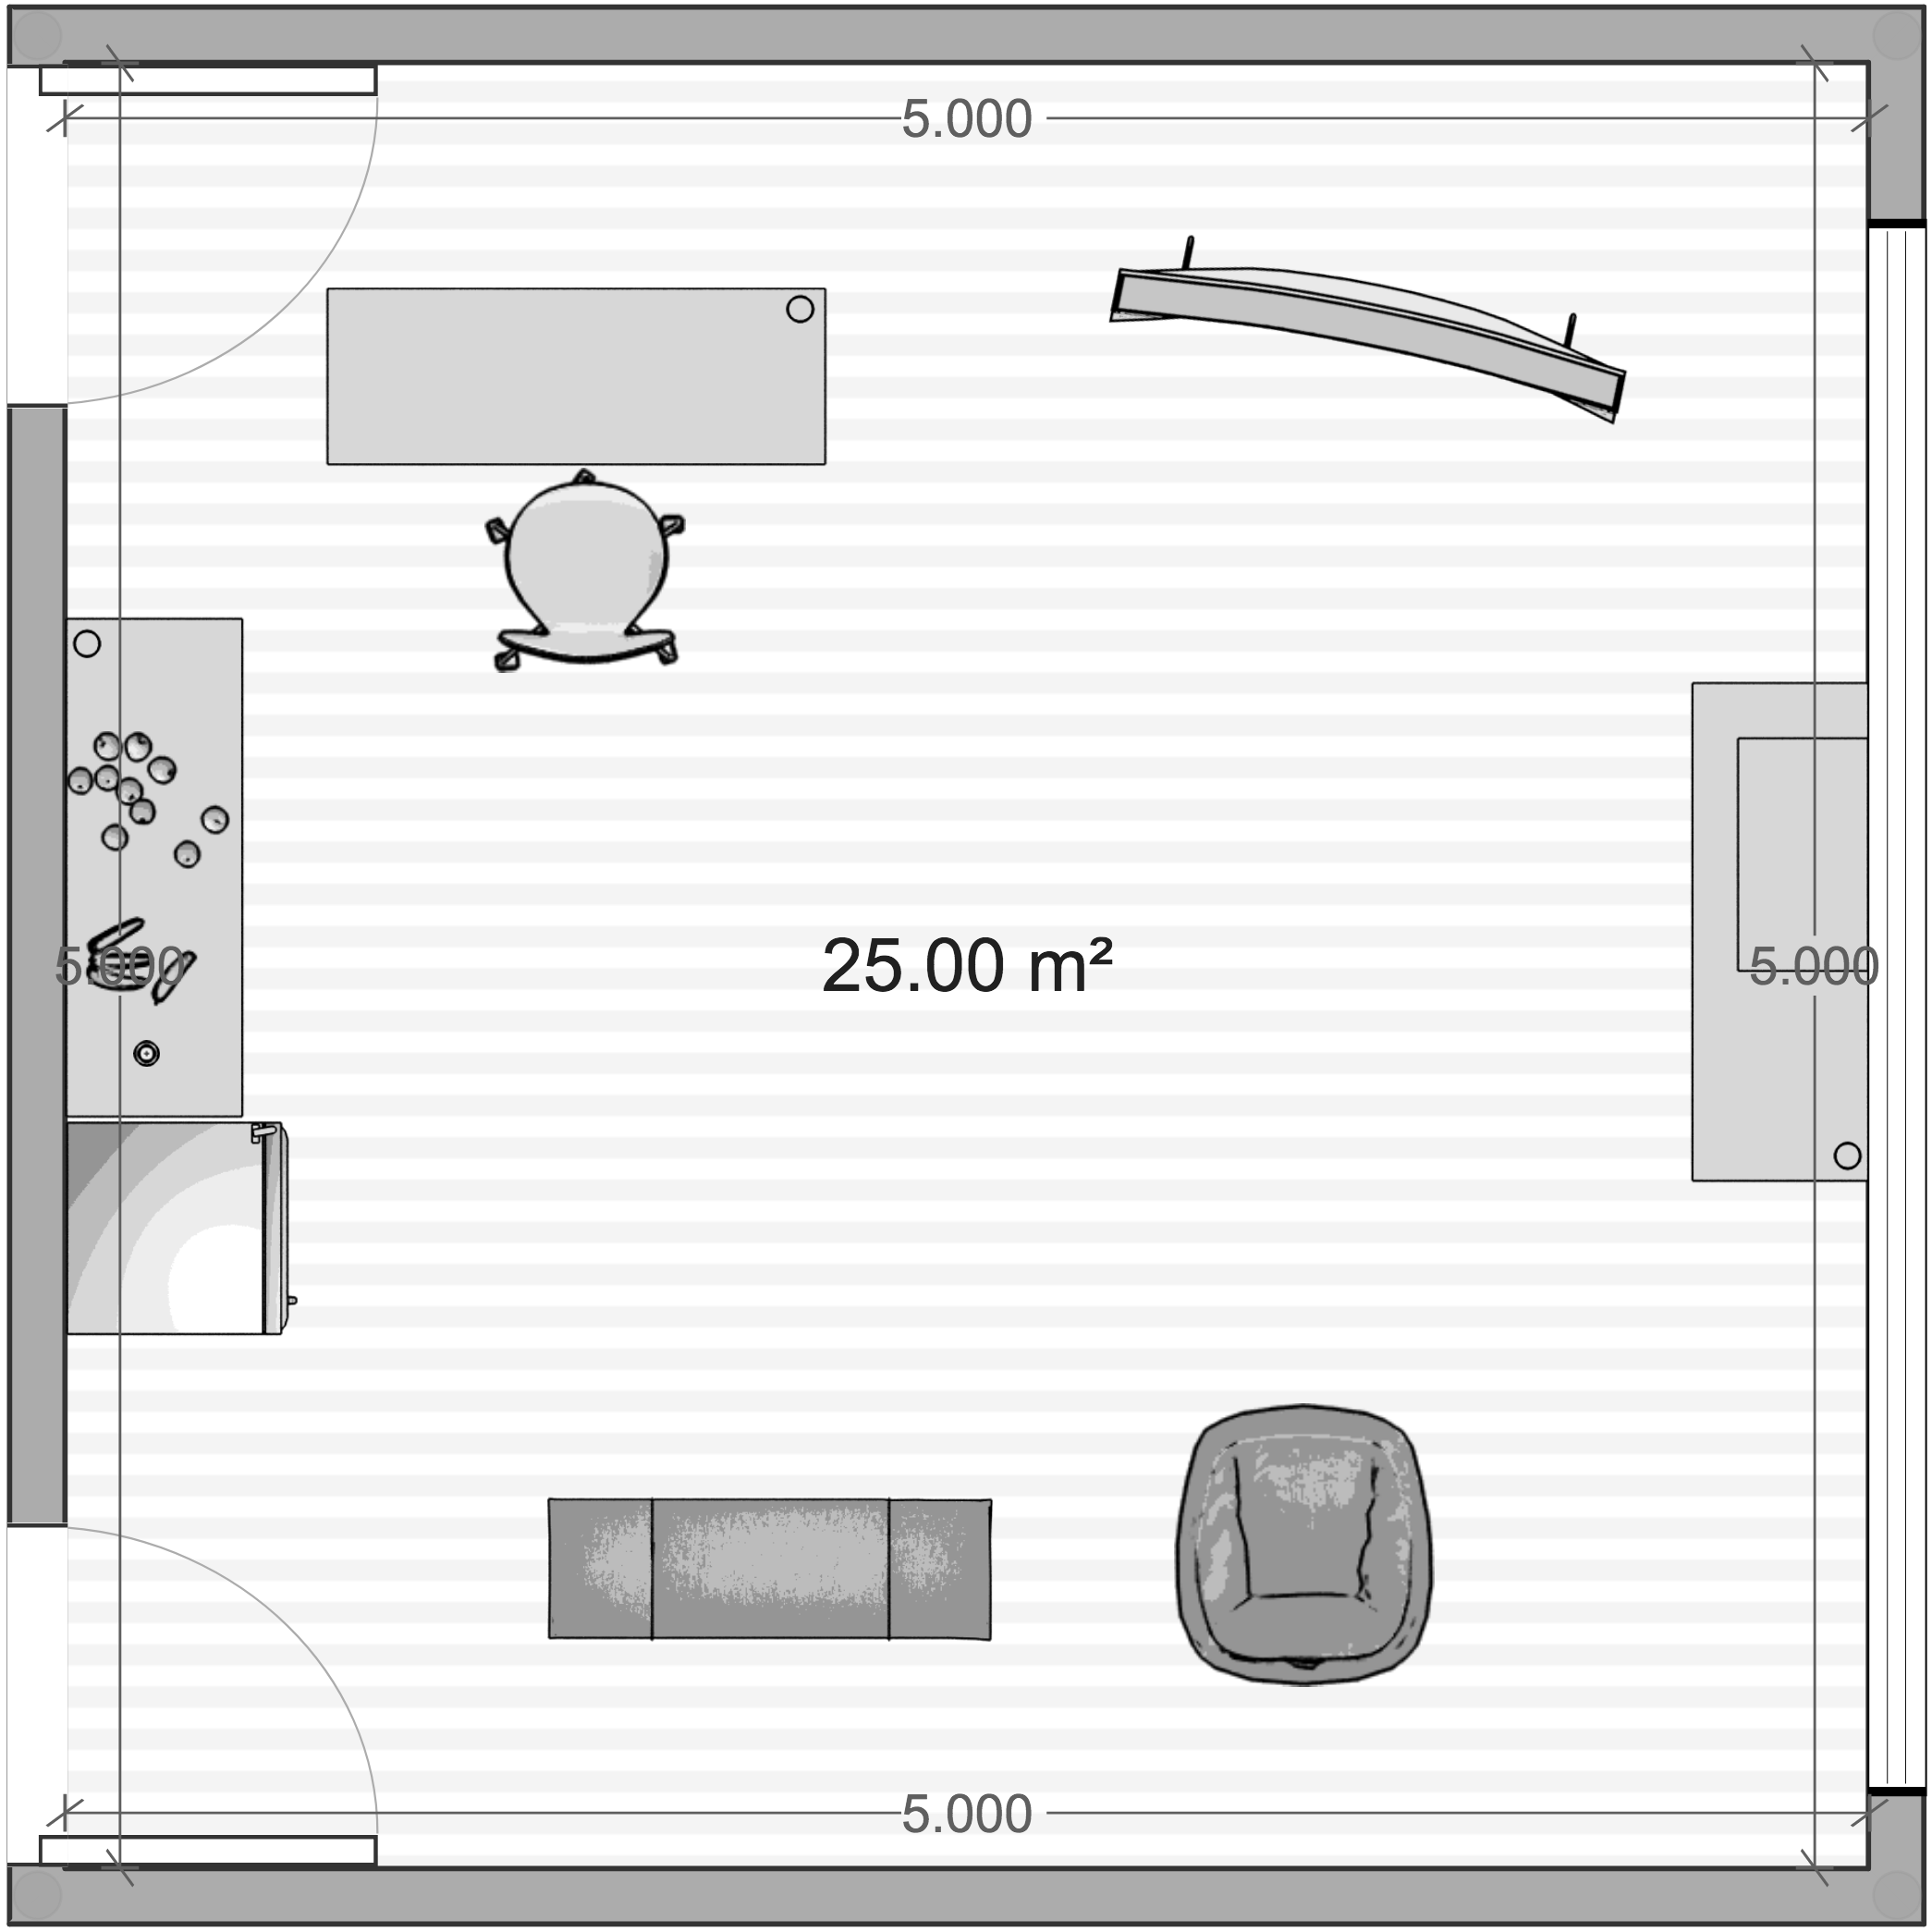
\includegraphics[width=0.6\textwidth]{images/floorplan}
\caption{집안 거실을 모사한 실험 장소의 평면도}
\label{fig:floorplan}
\end{figure}
%%%%%%%%%%%%%%%%%%%%%%%%%%%%%%%%%%%%%%%%%%%%%%%%%%%%%%%%%%%%%%%%%%%%%%%%%


\subsubsection{인간참여형 \sysname\ 시스템}

본 사용자 스터디에서는 \ref{sec:system_implementation}에서 언급했듯이 \cite{kang2018homemeld}에서 제시한 \sysname\을 인간 참여(Human-in-the-loop) 형태로 바꾸어서 오즈의 마법사(Wizard-of-Oz) 실험을 진행했다.

실험을 위해 텔레프레즌스 로봇의\cite{double_robotics} 조종 경험이 있는 두명의 조종사를 모집했다. 먼저 각 방에 설치된 스마트폰을 통해 각 방에 어디에 사람이 위치하는 지 영상을 관찰했다. 이후 각 조종사는 텔레프레즌스 로봇 조종 프로그램을\cite{double_drive} 통해 각 로봇을 동일한 위치로 움직였다. 로봇의 방향의 경우 상대방을 바라보고 있는 지 여부를 동기화하는 데 집중했다.

텔레프레즌스 로봇 사이는 음성 통화(FaceTime)로 연결하여 서로의 목소리 및 생활 속 일상 소음이 서로 전달 될 수 있도록 했다. 텔레프레즌스 로봇의 화면은 사용하지 않았다. 방향이 제대로 맞지 않으면 의미 있는 정보 전달이 이루어지지 않고, 로봇을 따라다니면서 화면을 보는 경우를 막기 위하여 화면은 띄우지 않는 방향으로 통제하기로 결정했다.


\subsubsection{사전 인터뷰}

사전 인터뷰는 커플의 인구학적 특성과 함께함의 형태 및 경험의 깊이에 대한 질문으로, 시스템 체험 전에 30분 동안 진행했다. 인터뷰에서 물어본 핵심 질문들은 다음과 같다. ``두 사람은 얼마나 오래 알고 지냈나요?'', ``함께 살기 시작하고 나서 상대방에 대해 더 잘 이해하게 되었다고 생각하시나요?'', ``평소에 집에 두 분이 함께 계시는 시간은 어느정도 되나요?'', ``같이 계실때면 두 분은 서로 어떻게 시간을 보내시나요?'', ``상대방이 피곤하다고 느끼신 적이 있나요?''. 자세한 핵심 질문 목록은 표 \ref{tab:userstudy_pre_questionnaire}에 나열했다.


%%%%%%%%%%%%%%%%%%%%%%%%%%%%%%%%%%%%%%%%%%%%%%%%%%%%%%%%%%%%%%%%%%%%%%%%%
\begin{table}
	\centering
	\caption{사전 인터뷰 핵심 질문 목록}
	\label{tab:userstudy_pre_questionnaire}
	\newcommand{\mr}[2]{\multirow{#1}{*}{#2}}
	\begin{tabular}{ll}
		\toprule
		\textbf{주제 (Theme)} & \textbf{종자 질문 (Seed Questions)} \\
		\midrule
		\mr{3}{``함께 삶''의 깊이}
		& 두 사람은 얼마나 오래 알고 지냈나요? \\
		& 함께 살고 있다는 확연히 느낀 순간이 있나요? \\
		& 함께 살기 시작하고 나서 상대방에 대해 더 잘 이해하게 되었다고 생각하시나요? \\
		\midrule
		\mr{2}{``함께 삶''의 형태}
		& 평소에 집에 두 분이 함께 계시는 시간은 어느정도 되나요? (주말 / 주중) \\
		& 같이 계실때면 두 분은 서로 어떻게 시간을 보내시나요? \\
		\midrule
		\mr{5}{``함께 삶''의 요소}
		& 함께 있을 때 아직 서로가 신경쓰이시나요? \\
		& 상대방이 피곤하다고 느끼신 적이 있나요? \\
		& 배려 받고 있다고 느끼신 적이 있나요? \\
		& 보통 대화를 어떻게 시작하시나요? \\
		& 말을 하지 않아도 함께 하실때는 서로의 기척을 잘 느끼시는 편인가요? \\
		\bottomrule
	\end{tabular}
\end{table}
%%%%%%%%%%%%%%%%%%%%%%%%%%%%%%%%%%%%%%%%%%%%%%%%%%%%%%%%%%%%%%%%%%%%%%%%%


\subsubsection{시나리오 체험}

시나리오 체험의 목적은 영상 통화 혹은 \sysname\이 제공되는 상황에서 \concept\가 어떻게 형성되는 지 참가자가 실제 체험해볼 수 있도록 하는 것이다. 그 과정을 돕기 위해 우리는 \concept\를 체험할 수 있는 적절한 시나리오를 제공하고자 했다.

시나리오 체험 세션은 15분의 길이를 가지는 3개의 세션으로 이루어졌다. 각 세션에서는 차례로, 서로 함께 있는 상황, 텔레프레즌스 로봇 아바타를 통해 소통하는 상황, 영상통화(Skype)를 통해 소통하는 상황을 체험했다. 자연스러운 환경을 위해 체험 중에는 실험 참여자들만 실험방에 위치하도록 했다. 연구자는 각 세션의 사이에 다음 실험을 위해 환경을 바꿀때만 출입하였다.

실험을 위한 시나리오를 기획하는 과정에서 가장 중요하게 고려한 요소는 어떻게 참가자들이 ``\concept''에 빠지도록 할 수 있을까였다. 우리는 두 사람이 조용한 환경에서 각자 자신의 할 일에 집중하고 있는 상황을 선택했다. 각자 할 일에 집중하고 있는 상황은 서로 대화가 잦지 않으며 서로 얼굴을 바라보지 않아도 괜찮다. 또한 주변 소리가 없는 고요한 환경에서 진행해도 어색함이 없으며, 움직임이 많지 않다. 이들 요소는 텔레프레즌스 로봇의 외형이 가지고 있는 여러 요소들의 영향을 통제할 수 있게 해주었다. 대면을 요구하지 않는 상황은 영상 통화의 필요성을 제거해 주었고, 배경 음악이 존재할 때 생기는 불편한 소음 또한 조용한 환경이기에 배제할 수 있었다.

실험 참가자들이 각자 할 일을 선정할 때는 다음과 같은 요소를 고려했다. (1) \textit{일상적이지만 명확한 할 일.} 실험 환경은 실제 살아가는 환경이 아니기에 일상적인 활동에 자연스럽게 빠져들기 힘들다. 이 문제를 해결하기 위해 우리는 실험 참가자들에게 미리 할 일을 들고 와달라고 부탁했다. 참가자들이 제시한 할일의 예시에는 시험 공부, 드라마 시청, 여행 계획 세우기 등이 있었다. (2) \textit{할 일의 집중도에 차이를 주기.} 두 사람에게 명확히 할 일을 정해주었을 때 두 사람 사이의 소통이 너무 적어지는 문제가 발견되었다. 집중도가 높아 소통의 빈도가 너무 떨어지면 15분 동안 \concept\를 충분히 체험할 수 없었다. 이를 해결하기 위해 우리는 할 일을 정해줄 때 적어도 한 사람은 집중이 많이 필요하지 않은 할 일을 하도록 제한했다. 예를 들어, 한 사람이 시험 공부 등 집중을 많이 요구하는 일을 하면, 다른 사람은 책을 읽거나 드라마를 보는 등 편한 활동을 하도록 했다. 각 커플이 진행한 활동은 표 \ref{tab:userstudy_activity}에 나열했다. 집중도가 높다고 판별한 활동은 이탤릭체로 표시했다.

마지막으로 텔레프레즌스 로봇이 사용자들에게 익숙한 기기가 아니라는 문제가 있었다. 텔레프레즌스 로봇에 대한 지나친 관심은 참가자들이 객관적으로 시나리오를 체험하지 못하게 만들 수 있다(Novelty Effect). 따라서, 우리는 시나리오 체험 전에 텔레프레즌스 로봇에 대한 노출을 최대화 하고자 했다. 사전 인터뷰 때 부터 사용자가 텔레프레즌스 로봇과 함께 위치하도록 했으며, 시나리오 체험 세션에 들어가기 전에 로봇이 어떻게 동작하는 지 직접 확인해 볼 수 있는 5분 정도의 소개 시간을 가졌다.


%%%%%%%%%%%%%%%%%%%%%%%%%%%%%%%%%%%%%%%%%%%%%%%%%%%%%%%%%%%%%%%%%%%%%%%%%
\begin{table}
\centering
\caption{각 커플이 시나리오 체험을 위해 선택한 활동 목록}
\label{tab:userstudy_activity}
\begin{tabu}{cc}
	\toprule
	\rowfont[c]{\bfseries}
	커플 & 활동 \\
	\midrule
	가 & \emph{시험 공부}, 책읽기 \\
	나 & 스마트폰으로 야구 시청, 책읽기 \\
	다 & 책읽기, 그림 그리기 \\
	라 & 스마트폰 게임, 드라마 시청 (스마트폰) \\
	마 & 여행 관련 도서 읽기, \emph{여행 계획 작성하기} \\
	\bottomrule
\end{tabu}
\end{table}
%%%%%%%%%%%%%%%%%%%%%%%%%%%%%%%%%%%%%%%%%%%%%%%%%%%%%%%%%%%%%%%%%%%%%%%%%


\subsubsection{사후 인터뷰}

사후 인터뷰에서는 실제 실험에서 관찰한 내용을 중심으로 구체적인 상황에 대한 실험 참가자의 주관적인 해석을 수집했다. 인터뷰 질문의 핵심 테마에는 쌍방의 존재에 대한 인식, 주의의 배분, 서로의 행동 사이의 연관성 등이 있었다. 이들 테마는 소셜 프레즌스(social presence) 측정하는 설문지\cite{biocca2001networked}에서 \concept와 관련된 개념을 중심으로 선택하였다.


\subsection{실험의 어려움 및 한계}

\yjc{이 단락, 쓸 필요가 있을까요? 지워버릴까...}

본 단락에서는 실험 디자인 과정에서의 어려움 및 한계에 대해 간략히 논한다.

\subsubsection{왜 정성적 연구인가}

우리는 본 실험을 통해 \sysname\이 실제 \concept\를 재현하는 순간들을 정성적인 방법론을 통해 포착하고자 했다. 그 이유에는 크게 두가지가 있다. 먼저 \concept와 관련된 요소들을 측정할 수 있는 적합한 심리학/사화과학적 지표를 찾을 수 없었다. 소셜 프레즌스(Social Presence)과 관련된 지표\cite{biocca2001networked}가 가장 가까웠지만, 우리가 제안하는 \concept와는 차이가 있었다. 개념적으로 가까운 사람의 주변인지(Pheripheral Presence), 주변-코프레즌스(Ambient co-presence) 관련 논문들도 찾아보았지만, 실험을 통해 주장을 뒷받침하고자 한 예시를 찾기 어려웠다.

둘째로, 정량적인 실험을 디자인 하기에는 \concept에 대한 지식이 부족하다고 판단했다. 정량적인 실험을 하기 위해서는 실험하고자 하는 조작 변인 외의 통제 변인에 대해서는 정교한 설계가 필요하다. 하지만 어떤 요소가 핵심적이고 \concept에 어떻게 영향을 끼치는 지 모르기에 해당 실험 환경을 구성할 수 없었다.


\subsubsection{왜 연구실 환경에서 실험했는가}

\sysname의 효과를 가장 잘 확인할 수 있는 방법은 실제로 떨어져 살아가는 커플의 집에서 실험을 진행하는 것이다. 하지만 실험 대상 모집의 문제로 우리는 연구실 환경에서 시나리오 기반 실험을 진행했다. 실제 \concept\가 어떻게 이루어지는 지 확인하기 위해서는 적어도 다섯 커플에 대한 실험이 필요하다고 생각했다. 또한 떨어져 사는 감정을 체험하기 위해서는 실제 물리적으로 떨어진 곳에 두 집을 가지고 있어야 했으며 집의 구성 또한 로봇이 움직일 수 있는 형태여야 했다. 해당 조건을 만족하는 다섯 커플 찾고, 이들의 실제 집을 빌려서 실험을 진행하는 것은 시간적으로나 금전적으로나 부담이 컸다.

추후 실험에서는 실제 떨어져 살고 있는 커플에게 \sysname\을 오랜 시간 체험할 수 있도록 하는 장기 사용자 스터디(Long-term user study)를 진행하고자 한다.


\section{실험 결과}

% 모든 참가자를 아우르는 전반적인 테마
% <상대방에 대한 이해의 중요성>

모든 참가자들은 함께 살아가면서 생기는 상대방의 습관에 대한 깊은 이해를 연애 시절과 달라진 가장 큰 변화로 뽑았다. 커플 \texttt{가}는 가까운 기숙사에 살며 오랜시간 연애를 했지만, 함께 살기 시작하면서 언제 더럽다 느끼고 청소를 시작하는 지, 생활에서 민감하게 생각하는 요소가 무엇인지 등 맞춰갈 점이 많았다고 말했다. 커플 \texttt{나} 또한 남편이 빨래를 돌리는 횟수가 무척 많아서 놀랐다는 얘기를 해 주었다.

그러나 상대방에 대한 깊은 이해를 바탕으로 한 은근한 함께 삶을 친밀감을 주는 핵심 요소로 뽑는 사람은 많지 않았다. 참가자들은 파트너와 깊은 대화를 나누는 시간을 함께 삶에 가장 중요한 요소로 뽑았다. 커플 \texttt{가}는 함께 식사를 하는 시간을, 커플 \texttt{마}는 자기 전에 대화를 나누는 순간을 함께 살아간다고 느끼는 순간으로 뽑았다.

하지만, 모든 참가자들은 이러한 대화의 순간은 일상 속에서 흔하지 않다고 언급했다. 커플 \texttt{가}의 남편은 ``대화하는 스위치가 눌렸을 때만'' 대화를 한다면서 대표적 순간으로 ``밥을 다먹고 설거지 하기 전, 다 씻고 침대에 누웠을 때''와 같은 상황을 제시했다. 커플 \texttt{다}의 남편은 ``대부분의 대화는 `이거 봐봐', `저것 좀 해줘'입니다''라며 깊은 토론은 상황이 받춰줄 때만 진행된다고 언급했다.

비록 참가자들은 \concept\가 함께 살아가는 두 사람 사이의 친밀감의 직접적인 원인이 아니라고 말했지만, 우리는 지속적인 상황의 공유가 두가지 측면에서 함께 삶을 형성하는 데 도움을 줄 수 있다고 생각했다. 첫째, 깊은 대화를 시작할 수 있는 순간을 찾아주는 데 도움을 줄 수 있으며, 둘째, 가벼운 신볍잡기식의 얘기가 더 자연스럽게 나올 수 있는 환경을 제공해줄 수 있다. 이에 맞추어 우리는 본 실험 결과를 해석하는 데 있어 \approach의 제공이 소통의 환경이 어떻게 변화시키고 이것이 \concept와 어떻게 연결되는지를 서술하는데 집중하였다.

% 이후 나올 관찰 결과들 Outline 하기
본 절에서 설명할 관찰 결과들은 다음과 같다. 먼저 사전 인터뷰를 통해 떨어져 사는 사람들의 경우 적은 정보로도 상대방의 상태를 파악하고자하는 적극성이 함께 살아가는 사람들보다 더 크다는 사실을 확인할 수 있었다. 함께 살아가는 사람들의 경우, 전화 등이 없어도 쉽게 상대방의 상태를 파악하고 얘기할 수 있기에, 상대방의 상태를 유추해야하는 필요성을 그다지 느끼지 못했다. 우리가 제안한 \sysname에 있어서는 대화의 공백에 대한 적은 부담감, 특정 위치에서 들려오는 목소리, 로봇의 움직임이 주는 대화의 기회에 대해 긍정적인 반응을 보여주었다.


\subsection{은근한 상황 정보 획득에 대한 적극성}

\begin{quote}
``제가 비밀번호 누를 때 소리를 아니까 띠띠띠띠 하면 `들어 갔네' 그러고, (남편은) `뭐 눈달려있나' 하고요. \ldots 또 연구실에 집까지 걸 어서 얼마나 걸리고, 자전거 타고가면 얼마나 걸리고 대충 아니까, 막 시끌벅적하면 아 거기쯤 지나가나 보네 하고.'' --- 여자, 커플 나
\end{quote}

사전 인터뷰에서는 기존의 삶에서 함께함이 어떻게 나타났는지 구체적인 경험을 뽑아내고자 했다. 그 중 하나는 상대방의 현재 상태를 어떻게 알아내는 지에 관한 질문이었다.

상대방의 상황를 알고자 하는 의지와 그 수준은 커플마다, 그리고 개인마다 차이가 났다. 커플 \texttt{나}의 여자는 남편의 현재 상황를 알아내는 방법에 대해 위와 같이 상세하게 묘사를 했지만, 커플 \texttt{가}의 남자는 ``저는 (와이프가) 잘 몰라줘서 그냥 직접 말해줘요. `나 오늘 피곤해' 이렇게'' 라고 말했다. 커플 \texttt{마}의 남자는 눈치가 없어서 명확히 말해주기 전에는 잘 몰라서 구박을 많이 받는다고 표현했다.

특히 떨어져 생활하는 시간이 있는 커플 \texttt{가}와 \texttt{나}, \texttt{라}들은 전화 통화를 할 때 있어 상대방의 상황을 아는 것은 매우 중요하다는 의견을 얘기했다. 이는 전화 통화가 가능한 상황을 판별하고, 대화의 길이를 조정하기 위해서였다. 이들 커플들은 공통적으로 퇴근 시간을 합의된 대화 시간으로 언급했다. 대학원생 커플 \texttt{가}의 경우, 보통 연구실에 있을 때 전화통화를 하기에 전화에서 들리는 주변 소음에 따라 연구실에서 통화하는 지, 복도에서 통화하는 지 알고 전화 시간을 조절한다고 언급했다.

이와 반대로 현재 함께 살고 있는 커플 \texttt{다}와 \texttt{마}의 경우 상대방의 상태 파악에 큰 필요를 표현하지 않았다. 두 커플 모두 업무 시간 동안에는 거의 통화하지 않는다고 했으며, 상대방의 상태를 파악하기 위해 유심히 관찰한 적이 없다고 얘기했다. 커플 \texttt{마}의 여자는 현관문을 보는 모습만 보아도 오늘 피곤한지 아닌지 파악이 가능하다고 언급했다. 그렇다고 해서 두 커플이 상대방의 상태에 맞추어 주려는 노력이 없지는 않았다. 커플 \texttt{다}는 상대방이 피곤할 때는 말하기 전에 설거지를 미리 해두는 등 대화를 하지 않아도 될 상황을 만들어 준다고 말했다. 커플 \texttt{마} 또한 기분이 안 좋아 보일 때면, 상대방의 신경을 거스르지 않도록 노력한다고 얘기했다.

이와 같은 결과는 함께 사는 사람들과 떨어져 사는 사람들 사이의 환경의 차이에 따른 결과로 보인다. 상대방의 상황에 맞추어 대화의 수준과 빈도를 조절하는 노력은 모든 커플이 공통적으로 언급했지만, 이를 위해서 한 구체적인 노력에 대한 질문의 대답은 주말 부부와 함께 사는 부부 사이에서 많은 차이가 났다. 떨어져 사는 커플의 경우 예시를 들며 활발히 얘기했지만, 함께 사는 부부는 구체적인 예시를 찾지 못했다.

함께 사는 커플의 경우 다양한 통로를 통해 상대방의 상태를 인식하고 있고 같이 있는 동안에는 자유로운 대화가 가능하다. 반대로 떨어져 사는 커플에게 전화 통화는 유일한 연결 통로다. 그렇기에 들려오는 주변 정보를 통해서 민감하게 상대방의 상황을 파악하고 그 상황에 맞추어 전화 통화를 진행해야한다는 부담이 있다.  전화\textperiodcentered영상 통화가 제공하는 정보 전달 능력은 통화 상황에만 한정되어 있고, 통화 전후 상황에 대한 정보 전달은 전혀 없기 때문에 전화를 걸기 전, 그리고 통화를 진행하는 중간에도 부담을 많이 느끼게 된다. 이와 같이 음성\textperiodcentered영상 통화가 가지고 있는 전화 걸기의 부담감은 대화의 빈도나 깊이에 영향을 끼치고, 결과적으로 은근한 함께 삶을 느끼는 데 있어 부정적인 요소로 작용할 수 밖에 없다.


\subsection{대화의 공백에 대한 적은 부담감}

\begin{quote}
``Skype는 내가 뭐하고 있다 하면서 보여줄라니까 에너지가 많이 들고 디스트랙트가 많이 됐구요, 세번째(\sysname)는 이미 얼굴을 보고 있지도 않고 옆에서 움직이는 사람을 신경쓰지 않아도 되고, 내가 할 거 하는데 가장 좋았어요.'' --- 여자, 커플 다

``오히려 화상 통화 할 때는 얼굴을 계속 봐야되서 붙어 있어야만 했지만 로봇은 그렇지 않아서 항상 같이 있어야 될 필요는 못 느꼈어요.'' --- 남자, 커플 다
\end{quote}

또한 참가자들은 영상 통화가 강제하는 얼굴 마주보기에 대해 부담감을 표현했다. 위의 표현을 한 커플 \texttt{다}의 여자는 벽면 화이트 보드에 그림을 그리면서 대면을 하기 위해 끊임없이 책상과 화이트보드 사이를 왔다갔다 했다. 벽면을 보고 있을 때는 화면을 같이 볼 수 없기 때문에 혹시 상대방이 어떤 표현을 했는 데 놓치는 것이 있을까봐 그랬다고 참가자는 설명했다. 이어 ``함께 있는 상황에서는 눈을 꼭 마주치면서 이야기를 하지는 않는다는 것을 알게 되었다''고 말했다. 커플 \texttt{마}는 얼굴을 마주보지 않아서 생긴 오해의 순간도 있었다고 언급했다.

\begin{quote}
남자: ``(제가) 책을 보고 있었는데, 아내가 보기에는 눈을 마주치지 않아서 (마치 내가) 눈을 피한다고 생각을 한 것 같아요.''

여자: ``아 그게 어떤 상황이냐면, (상황 설명), 그 얘기를 하고 나서 내 표정이 안좋았고, 뭔가 책을 보고 있으니까 그 상황에선 남편이 꼭 내 시선을 피하는 것 처럼 느껴졌다. 그래서 ‘왜 내 눈을 안쳐다보지?’ 하는 대화가 오간 상황이었어요'' --- 커플 마
\end{quote}

영상 통화 중의 대화의 공백에 대한 불안감도 있었다. 커플 \texttt{라}의 경우, 영상 통화 세션 내내 ``지금 뭐해''와 같은 질문을 지속적으로 던졌다. 커플 \texttt{마}의 남자는 통화의 경우 상대방에게 모든 신경을 써야 한다는 부담감 때문에 지속적으로 대화를 시도했다고 언급했다. 이와 같은 대화의 공백에 대한 불안감은 이전 연구\cite{mclaughlin1982awkward}에서도 언급된 바 있다.

일부 참가자들은 이러한 요소가 제안하는 \sysname 시스템에서는 훨씬 덜했다고 말했다. 커플 \texttt{가}는 시험 공부하는 상황에서는 시야에 로봇이 존재하지 않아 신경을 쓸 필요가 없었다고 말했다. 커플 \texttt{마}의 남자는 \sysname\을 비디오 챗 시스템으로 생각하고 로봇 앞에 앉아 있었고, 화면이 나오지 않아서 힘들었다고 언급했다. 하지만 커플 \texttt{마}의 여자는 해당 세션이 가장 집중하기 좋았던 세션이라고 언급했다.

이는 실제 주어진 활동의 진행량에 있어서도 차이를 보여주었다. 진행량의 비교가 쉬운 커플 \texttt{나}의 여자(책읽기)와 \texttt{다}의 남자(책읽기), \texttt{마}의 여자(여행 계획 작성)에게 각 세션 별로 언제 가장 진행이 많이 되었냐고 물어보았을 때, 모두 \sysname\ 상황에서 가장 많은 양의 책을 읽고, 노트를 작성했다고 말했다.

\yjc{해석 추가하기}
%\approach\가 추구한 물리적인 존재감은 상대방과 함께하고 있다는 사실을 적은 주의 배분으로도 전달할 수 있는 수단으로 보인다. 영상 통화의 경우 서로 얼굴을 바라보고 대화를 진행해야만 상대방이 나와 함께 있다는 느낌을 전달할 수 있다.


\subsection{상대방의 위치에서 들려오는 목소리}

\begin{quote}
``\ldots 소리가 어느 방향에서 들려온다가 다른 걸 할 때에 큰 차이를 주는 것같아요. \ldots 그 위치에서 소리가난다는 것은 (안 보고 있으면 그게 사람인지 아닌지 뭔지 모르지만) 익숙한 목소리가 그 방향에서 들려오니까 같은 공간에 함께 있을 때를 모사할 수 있어보여요.'' --- 남자, 커플 다
\end{quote}

참가자들은 특정 위치에서 들려오는 목소리에 대해서 긍정적인 평가를 주었다. 특히 해당 요소가 공간감, 그리고 함께 있는 느낌에 큰 효과를 주었다고 표현했다. 커플 \texttt{다}는 공간 속에서 들려오는 소리는 일반 헤드폰으로 듣는 소리와 큰 차이가 있다면서 (남자), 특정 위치에서 들려오는 소리가 나와 같은 공간에 아바타가 있는 느낌을 준다고 언급했다 (여자). 커플 \texttt{가}의 남자는 해당 아이디어를 확장하여, 음성 통화도 특정 위치에서 들려오는 형태로 구현하면 좋겠다고 얘기했다.

\yjc{해석 추가하기}


\subsection{로봇의 움직임이 주는 대화의 기회}

\begin{quotation}
(여자는 빈백에 있다. 남자는 책상 의자에 앉아 로봇을 바라본다. 그림 \ref{fig:userstudy_scene} 참조.)

여자: ``난 엄청 가만히 있겠네?''

남자: ``어, 가만히''

(여자가 일어서서 부엌으로 이동한다.)

남자: ``어디가?''

여자: ``응? 나 뭐 마시려구.''

남자: ``야 이거 진짜 똑똑하다.'' --- 커플 라
\end{quotation}

모든 참가자들은 로봇의 움직임을 파악하는 것이 어렵지 않다고 얘기했다. 커플 \texttt{나}의 남자는 움직이는 그 현장은 못 보더라도, 로봇의 위치가 바뀐 것은 쉽게 알아볼 수 있다고 말했다. 

위에 적힌 커플 \texttt{라}의 대화는 로봇의 움직임을 통해 대화가 시작되는 가장 흔한 경우를 보여준다. 대화와 같이 집중도가 높은 행위 중이 아니라도, 로봇의 위치를 통해서 현재 상태가 계속 공유되기에, 상대방의 상태 변화의 순간을 즉각적으로 포착가능하다. 기존의 통화 방식에서는 대화는 시작하고자 하는 의지가 있어야만 가능했지만, \sysname\을 이용할 경우 상태가 지속적으로 공유되기에, 상태 변화에 맞추어서 말을 거는 것이 가능해진다. 이 요소는 음성\textperiodcentered영상 통화와의 큰 차이로, 대화의 시작에 대한 부담감을 줄여주어 \concept\ 형성에 큰 도움을 준다.

\yjc{해석 추가하기}

% 항상 나를 따라다녔으면 좋겠다.
% 대화에 관심을 가지고 있다는 증표가 남겨져 있으면 훨씬 편할 것 같다.

\yjc{\begin{itemize}
	\item 주말 부부 등 떨어져 생활하는 시간이 있는 사람들이 “은근한 함께함”을 형성 하는 데 더 적극적으로 노력했다.
	\item 영상 통화시 항상 대면을 해야한다는 부담감 (관찰, 말) -- 은근한 함께함(5)에 부정적
    \item 방 안 특정 위치에서 들려오는 소리에 의한 공간내 존재감 (말) -- 은근한 함께함(1) -- 해석 잘 하면 4번 까지.
    \item 로봇의 위치변화를 통해 상대방의 상태 변화를 인식 (관찰) -- 은근한 함께함(2)
\end{itemize}}
